\documentclass{IEEEtran}
\usepackage{graphicx}
\usepackage{amsmath}
\usepackage[utf8]{inputenc}

\title{Using Normalised Radial Based Functions (NRBF's) to Predict Energy Consumption in the National Grid}
\author{Connor Wheeler}
\date{11/01/2018}

\begin{document}
\pagenumbering{arabic}

\maketitle

%\tableofcontents
\newpage
\section{Introduction}
\begin{flushleft}
    Training a Neural Network to predict the energy Consumptions of the national was not the easiest of tasks
    for the network to preform. There a number of interesting occurrences in the data, the output of the network and
    the results of the sigma optimisation and node optimisation.
\end{flushleft}
\section{Network}
\subsection{NRBF}
\begin{flushleft}
  Normalised Radial Based Functions (NRBF) work by using the activation of all nodes in the hidden
  layer to work out the output of the network. This is done by using the Gaussian activation function
  of the nodes in the hidden layer, to work out how active the node is when a value is passed to it.
  if a node is very then its activation value will be one or very close to one, where as an inactive
  node will be much closer to zero. The activation of all of the nodes is later used to work out what
  the output of the net work will be.
\end{flushleft}

\begin{flushleft}
  When the activation has been calculated this can then be used to get the output of the network
  as the more active nodes will contribute more to the final value that is output based on these inputs.
  To do this the sum of the nodes weights multiplied by the activation of the node is calculated.
  This part of the equation can be seen in figure 1:
  \vspace{3mm}

  $$\sum_{n=1}^{N}W _n\phi(\|x-x_n\|) $$
  \\
  \vspace{1.5mm}

  {\footnotesize figure 1 : sum of all node activations multiplied by weights of all nodes}

  \vspace{3mm}
  After this the total sum of all node activations is calculated and summed. The equation for this
  can be seen figure 2.

  \vspace{3mm}

  $$\sum_{n=1}^{N}\phi(\|x-x_n\|) $$
  \\
  \vspace{1.5mm}

  {\footnotesize figure 2 : sum of all node activations}
  \\
  \vspace{3mm}
  When these have been calculated the 2 values are divided. to get the final output from the
  hidden layer. The whole equation can been seen in figure 3.

  \vspace{3mm}

  $$f(x)=\frac{\sum_{n=1}^{N}W _n\phi(\|x-x_n\|)}{\sum_{n=1}^{N}\phi(\|x-x_n\|)}$$
  \\
  \vspace{1.5mm}

  {\footnotesize figure 3 : sum of all node activations multiplied by weights of all nodes
  divided by sum of all node activations}
  \\
  \vspace{3mm}

\end{flushleft}

\begin{center}
  Node Activation Equation
\end{center}
\begin{flushleft}
  The node activation equation is used to calculated the activation of the node. if the value before
  the exponential is calculated is 0 then the activation of the node will be 1.
\end{flushleft}
$$y=exp(-\frac{1}{2\sigma^2} \sum_{k=1}^{K}(x_{k} - w_{jk})^2) $$
{\footnotesize figure 4 : Gaussian activation equation for NRBF nodes}
\begin{center}
  Root Mean Squar Equation
\end{center}
\begin{flushleft}
  The Root Mean Square equation is used to calculated how incorrect the network was with its output. This was
  used to compare different sigma's to see which has preformed the best on the testing data set.
\end{flushleft}
$$RMS =\sqrt{\frac{1}{M}\sum_{i=1}^{M}(y^{p}_{i} - y^{p}_{id})^2} $$
{\footnotesize figure 5 : Root Mean Square equation for calculating the error of the network}
\begin{center}
Weight Update Equation
\end{center}
\begin{flushleft}
  The weight update equation is used to adjust the weights in the hidden layer. This will allow the network to
  become more accurate over time as the weights get adjusted more and more, as the network becomes more accurate
  these adjustments become smaller. To do this the old weight is added to using the learning rate ($\alpha$) multiplied
  by the target value - the networks output, multiplied by the activation of the node ($\phi$).
\end{flushleft}
$$ W  \leftarrow W + \alpha *(target - Network output)*\phi$$
{\footnotesize figure 6 : Weight update equation used in the NRBF}
\subsubsection{Task 1}
\begin{flushleft}
 For task one an NRBF was made to work on a small and evenly distributed data set, to get the understanding of the network
 and the maths correct. To make sure the network was working correctly the sigma was set to 0.01 to see the step of the
 network function. this can be seen in figure 7. This was useful as it allowed to check if the network was working and
 was covering all of the training data points with the network function.
 \vspace{1.5mm}
\\
\vspace{1.5mm}
\begin{center}
  Network function with a sigma of 0.01
\end{center}
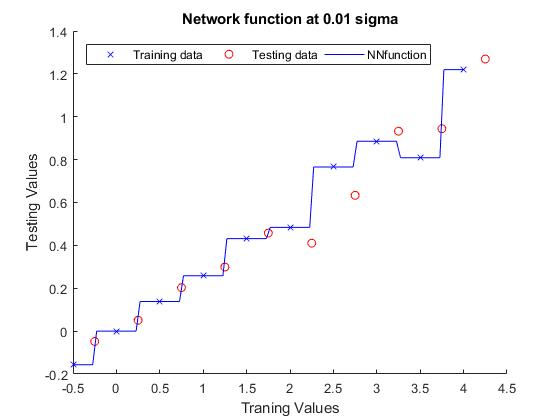
\includegraphics[scale = 0.35]{NNstepfunction.jpg}
\vspace{1.5mm}
{\footnotesize figure 7 : Network function when sigma is 0.01 }
\\
\vspace{1.5mm}
\end{flushleft}
\begin{flushleft}
  Once the network was working properly, the sigma optimisation could begin to see which sigma would be best to use for the
  network. To do this the network was run over the data set 100 times and then the final test and train error where taken and
  stored. This allowed for the best value on the testing data to be found. The sigma was tested between 0.1 - 1 and the table
  of results can be seen in figure 10. The best sigma value that could be found from this testing was 0.9 as it had the lowest
  test error of all of the value tried with a error value of 0.0915. The error graph and network function graph for this sigma
  can be seen in figure 8 and 9.
  \\
\vspace{1.5mm}
\begin{center}
  Error plot for a sigma of 0.9
\end{center}
\vspace{1.5mm}
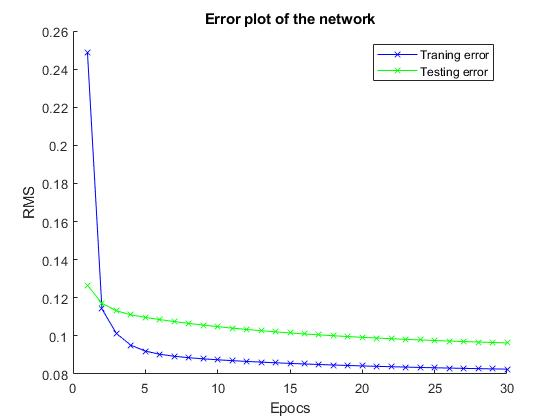
\includegraphics[scale = 0.35]{Errorplottask1.jpg}
\vspace{1.5mm}
{\footnotesize figure 8 : error plot for the network with sigma 0.9 }
\\
\vspace{1.5mm}
\begin{center}
  Network function plot for a sigma of 0.9
\end{center}
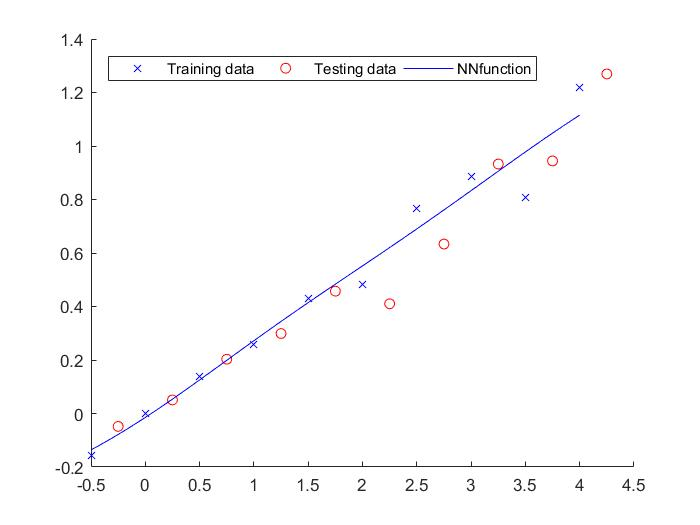
\includegraphics[scale = 0.35]{NNfunctiontask1.jpg}
\vspace{1.5mm}
{\footnotesize figure 9 : Network function when sigma is 0.9 }
\\
\vspace{1.5mm}
\end{flushleft}
\begin{center}
\begin{tabular}{||c c c||}
  \hline
Sigma Value & Train Error & Test Error \\ [0.5ex]
\hline
0.1 & 0.2733e-16 & 0.1005\\
0.2 & 2.0126e-10 & 0.1016\\
0.3 & 1.3562e-4 & 0.1094\\
0.4 & 0.0131 & 0.1161 \\
0.5 & 0.0439 & 0.1073 \\
0.6 & 0.0632 & 0.0983\\
0.7 & 0.0730 & 0.0933\\
0.8 & 0.0781 & 0.0919\\
0.9 & 0.0797 & 0.0915\\
1.0 & 0.0800 & 0.0918\\
\hline
\end{tabular}
\end{center}
\vspace{1.5mm}
{\footnotesize figure 10 : Sigma optimisation table }
\\
\vspace{1.5mm}
\subsubsection{Tast 2}

\begin{flushleft}
  For task 2 a NRBF that could predict the output of the national grid need to be made.
  This network would be much larger and more complex then the first one due to the fact that more
  data points would exist. When first creating and testing the network a node was used for each
  data point to check that every thing was working correctly, but this was not the best practice
  as some data points where very similar and could fit under one NRBF node.
  \\
  \vspace{2.5mm}
  So to lower the amount of nodes used in the hidden layer but still ensure that the nodes where
  evenly distributed K-means clustering was use to separate the data in to sets of clusters and then
  create the nodes. This meant that the number of nodes used would always be able cover the whole data set.
  This then allowed for testing in the form of node optimisation and sigma optimisation to get a much more
  efficient network. To get the number of nodes the total size of the data set is divided by a set number
  and that many nodes centres are then created. These node centres then used to set the centres of each node.
  As this network is a 3 dimensional network each node will be given 3 centres and have 3 input weight.
  \\
  \vspace{2.5mm}
  After the nodes have been created the input values are looped through by the network and each one is tested.
  After a data point has been tested the weights are updated and another data point is tested, after all the data point
  have been tested another epoc is run going through the data points again. This is done 100 times to allow
  for the larger sigma's to be trained by the network. The years 2012-2015 are used to train the network then the 2016
  data set is used for testing the network. 2017 data set is used to validate the network performance.
  \\
  \vspace{2.5mm}
  The network was trained across all of the training sets to allow for the network to be trained on all of the data
  available over those years and tested after each epoc. To ensure that the network was fully prepared for the
  final validation data set.
  \\
  \vspace{1.5mm}
  The graphs for all of this can be seen in the results section of this report

\end{flushleft}

\begin{center}
\begin{tabular}{||c c c||}
  \hline
Number of Nodes & Train Error & Test Error \\ [0.5ex]
\hline
0.1 \\
0.2 \\
0.3 \\
0.4 \\
0.5 \\
0.6 \\
0.7 \\
0.8 \\
0.9 \\
1.0 \\
\end{tabular}
\\
\vspace{2.5mm}
{\footnotesize figure 11 : Number of nodes compared to training error and
test error}
\end{center}
\begin{center}
\begin{tabular}{||c c c||}
  \hline
Sigma Value & Train Error & Test Error \\ [0.5ex]
\hline
0.1 \\
0.2 \\
0.3 \\
0.4 \\
0.5 \\
0.6 \\
0.7 \\
0.8 \\
0.9 \\
1.0 \\
\hline
\end{tabular}
\\
\vspace{2.5mm}
{\footnotesize figure 12 : Sigma optimisation of nodes the network based on the
best number of nodes}
\end{center}
\subsection{MLP}
\subsubsection{Task 2}
\begin{flushleft}
  MLP or Multi Layer Perceptron are a form of neural network that use sigmod activations
  to get an output based on all of the nodes in the hidden layer. Unlike NRBFS nodes in
  MLP's nodes don't have centres, and instead each node weight value is used to get a
  part of the final output. To get an output value from the network the sigmod activation
  is calculated from the input to the hidden layer. Then the hidden layer sigmod activation
  is calculated and passed to the output layer, where the total activation of all hidden
  nodes is calculated leading to the network output.
  \\
  \vspace{1.5mm}
  To optimise the MLP the number of nodes can be changed to see how this affects the overall
  output of the network. This can have a drastic change on the performance of the network, as
  the more nodes that are there the larger the impact the hidden node will have on the final
  network output. This has some problems as the nodes in the hidden layer will all be updated
  when the back propergation on the network takes place meaning that each node will be moved
  slightly based on the final output. This means that the MLP can never be 100\% accurate
  as its value is shifted every time so its best on the value that it has previously seen
  \\
  \vspace{1.5mm}
  The sigmod activation equation can be seen in the figure 13

$$y_i=\frac{1}{1+exp(-z_i)}$$
\\
\vspace{1.5mm}
{\footnotesize figure 13 : Sigmod activation function used in the MLP}
\\
\vspace{1.5mm}
When updating the weights in the network the delta rule is used to update all of
the weights in the network. the equation for this can be seen in figure 14.
$$W \leftarrow W  + \alpha*(y_i,_d - y_i)$$
{\footnotesize figure 14 : Delta rule weight update equation where $\alpha$ is the learning
rate}
\\
\vspace{1.5mm}

To optimise this network the max number of nodes was used and records of the error on training
and testing data was monitored and the number of nodes was slowly decreased over different tests
to see which amount of nodes would yield the best results.
\\
\vspace{1.5mm}
Along with this the learning rate was changed to see how this can affect the performance of the MLP.
 

\end{flushleft}
\section{Data}
\subsection{Data processing methods}
\begin{flushleft}
  For the network to use the data the average demand over each hour was taken and stored
  along with the day of the year, hour of day and the day of the week. This data was then
  normalised to be used in the network, to normalised the day the value would be divided by
  365. For example the first day of the year would be $1 / 365$. To normalised the hour the
  hour of the day was taken and then divided by 24. Finally the day of the week was divided
  by 7 to get a normalised set of numbers between 0 and 1.
  \\
  \vspace{1.5mm}
  Along with this the data processing could not factor in some of the data in the network, like
  the large spikes that occur from time to time and the leap years that also occur. These could
  of been factor in but then would also would of need to be factored in to the network when training
  leading to more problems.
\end{flushleft}
\subsection{Problems with the data}
\begin{flushleft}
  When processing the data there was a large array of problems that occurred. Some of the years of data where not
  complete and where missing entries over the year. Along with this the data reading where not always evenly sampled
  meaning some reading are very close to other where as others are very spaced apart. This is a very large problem when
  it comes to training to make the network as accurate as possible as the data might not reflect the height demands that
  could of occurred during the time of the reading. Along with this the data is sampled every 5 minutes, so to make the
  network as accurate as possible data would need to be taken more frequently and used to train the network.
  \\
  \vspace{1.5mm}
  Along with this some years will be leap years leading to the problem of there being 1 extra day for the network to
  learn that is not consistently there. This could be factored in to the network but would most likely only make a miner
  changer to the networks performance. Along with this there are spikes in the data where large world events had taken
  place or large sports events had taken place, this meant that more power was need and used as a result.
  This could be factored in to the network but there are so many edge cases and events that can not be predicted that
  it would most likely hinder rather then help the network to learn. Along with this cancelation of events or events only
  running every few years e.g. the Olympics would also need to be factored in and might lead to more energy being in the
  grid then is need.
\end{flushleft}
\section{results}
\section{conclution}
\end{document}
